\newpage
\begin{problem}
Шесть определений непрерывной функции.
\end{problem}
\begin{definition}
    Пусть функция $f$ определена на множестве E, точка $a \in E$. Функция $f$ называется непрерывной в точке $а$, если для любого $\varepsilon>0$ найдётся такое $\delta>0$, что при всех таких $x \in E$, что $|x-a|<\delta|f(x)-f(a)|<\varepsilon$.
\end{definition}

\begin{definition}
    Таким образом, определение непрерывной в точке $a$ функции можно записать и так: функция $f$ называется непрерывной в точке а, если точка а является изолированной точкой множества $E$, либо если $\lim _{x \rightarrow a} f(x)=f(a)(x \in E$ )
\end{definition}

\begin{definition}
    Так как стремление $x$ к $a$ происходит только по точкам множества $E$, то определение непрерывности допускает ещё одну формулировку: функция $f$ называется непрерывной в точке а, если точка а является изолированной точкой множества Е, либо если $\lim _{x \rightarrow a} f(x)=f\left(\lim _{x \rightarrow a} x\right)(x \in E)$
\end{definition}

\begin{definition}
    Учитывая определение бесконечно малой функции, мы можем записать определение непрерывности так: функция $f$ называется непрерывной в точке а, если точка а является изолированной точкой множества $E$, либо если
    $$
        f(x)=f(a)+\alpha(x)
    $$

    где $\alpha(x)$ - бесконечно малая функция при $x \rightarrow a, \alpha(a)=0(x \in E)$
\end{definition}

\begin{definition}
    В терминах окрестностей определение непрерывности примет вид: функция $f$ называется непрерывной в точке а, если точка а является изолированной точкой множества $E$, либо если для любого $\varepsilon>0$ справедливо следующее условие: $\varepsilon$-окрестность точки $f(a)$ содержит образ некоторой окрестности точки а при функции $f(x \in E)$ (определение непрерывности 5).
\end{definition}

\begin{definition}
    Если попытаться определить непрерывную функции с помощью определения предела по Гейне, то можно отказаться от того, что рассматриваются только последовательности, не принимающие значение $a$. Итак, используя определение предела по Гейне и его равносильность определению по Коши, получим ещё одно определение непрерывной функции: функиия $f$ называется непрерывной в точке а, если для любой такой последовательноcтu $\left\{a_n\right\}_{n=1}^{+\infty}$, ито $a_n \in E, a_n \rightarrow a, n \rightarrow+\infty, \lim _{n \rightarrow \infty} f\left(a_n\right)=f(a)$ (определение непрерывности 6).
\end{definition}

Отметим, что указывать отдельно на случай изолированной точки здесь не нужно, так как если последовательность со значениями во множестве $E$ стремится к изолированной точке $a$, то существует такое натуральное $N$, что $a_n=a$ при всех $n>N$.

\newpage
\begin{problem}
Определение непрерывности в точке справа и слева. Критерий непрерывности в терминах непрерывности слева и справа (Предложение 1, Лекция 13).
\end{problem}

\begin{definition}
    Функция $f: E \rightarrow \mathbb{R}$ называется непрерьвной справа в точке $a \in E$, предельной для $E_a^{+}$, если $\lim _{x \rightarrow a+} f(x)=f(a)$, и непрерывной слева, если $\lim _{x \rightarrow a-} f(x)=f(a)$ (здесъ точка должсна являться предельной для $E_a^{-}$.)
\end{definition}

\begin{proposition}
    $f \in C(a) \Leftrightarrow f$ непрерывна в а справа и слева, причём
    $$
        \lim _{x \rightarrow a+} f(x)=\lim _{x \rightarrow a-} f(x)=f(a)
    $$
\end{proposition}

\newpage
\begin{problem}
Локальные свойства непрерывных функций.
\end{problem}

\begin{proposition}
    (Локалъные свойства непрерывных функций). Пусть функции $f$ u $g$ определены на множестве $E, a \in E, f \in C(a), g \in C(a)$. Тогда выполнены следующие свойства:
    1) $\alpha f+\beta g \in C(a) \forall \alpha, \beta \in \mathbb{R}$ (линейная комбинация непрерывных в точке функций является непрерывной в этой точке функцией;
    2) $f \cdot g \in C(a)$ (произведение непрерывных в точке функций является функцией, непрерывной в этой точке);
    3) если $g(x) \neq 0 \forall x \in E$, то $\frac{f}{g} \in C(a)$ (частное непрерывных в точке функций является функцией, непрерывной в этой точке);
    4) $\exists M \geq 0, \delta>0: \forall x \in E \cap U_\delta(a)|f(x)| \leq M$ (для непрерывной в точке функции найдётся окрестность этой точки, в которой функиия ограничена);
    5) если $f(a) \neq 0$, то существует такая окрестность $U_\delta(a)$ точки а, что
    $$
        |f(x)|>\frac{|f(a)|}{2} \forall x \in E \cap U_\delta(a),
    $$

    причём для таких $x f(x) \cdot f(a)>0$, то есть функция $f$ совпадает по знаку с $f(a)$.
\end{proposition}


\newpage
\begin{problem}
Теорема о композиции непрерывных функций. Точка разрыва.
\end{problem}
\begin{proposition}
    (Теорема о композиции непрерывных функций). Пусть множества $E, D$ и K содержсатся в $\mathbb{R}, f: E \rightarrow D, g: D \rightarrow K$. Пусть $a \in E, f(a) \in D$, $u f \in C(a), g \in C(f(a))$. Тогда функция $g \circ f: E \rightarrow K$ непрерывна в точке а (здесъ $(g \circ f)(x):=g(f(x)))$.
\end{proposition}

\begin{definition}
    Если функция $f: E \rightarrow \mathbb{R}$ не является непрерывной в точке $a \in E$, то эта точка называется точкой разрыва функции $f$.
\end{definition}

\newpage
\begin{problem}
Устранимый разрыв, разрыв первого рода и разрыв второго рода. Разрывы монотонной
на интервале функции. Определение непрерывной на множестве функции.
\end{problem}
Во-первых, предел в точка $a \in E$ у функции $f$ может существовать, но не быть равным $f(a)$. В этом случае достаточно определить функцию $f$ в точке $a$ её пределом в этой точке, чтобы функция стала непрерывной, поэтому такая точка называется \textbf{точкой устранимого разрыва}. Примером функции с точкой устранимого разрыва может служить $f(x)=\frac{\sin x}{x}$, если $x \neq 0$ и $f(0)=0$, где $a=0$. Эта функция в точке $a=0$ имеет значение 0 , а предел при $x \rightarrow 0$ равен 1 , поэтому достаточно положить $f(0)=1$, чтобы функция $f$ стала непрерывной в точке 0 .

Во-вторых, в точке $a \in E$ у функции может не быть предела, но при этом существуют оба односторонних предела (см. предыдущую лекцию), которые не равны друг другу. В этом случае точка $a$ называется \textbf{точкой разрыва первого рода}. Иногда такой разрыв называют \textbf{скачком}. Примером функции с такой точкой разрыва может служить кусочно заданная функция $f(x)=\left\{\begin{array}{l}-1, \text { если } x<0, \\ 1, \text { если } x \geq 0 .\end{array}\right.$ Точка $a=0$ является точкой разрыва первого рода. См. также рис. 2 .

. \begin{figure}[h!]
    \center{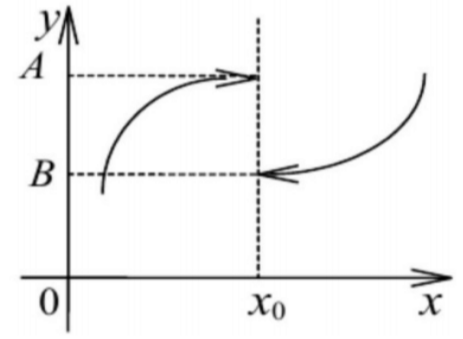
\includegraphics[scale=0.45]{Скачок.png}}
    \caption{Скачок величины $|BA|$.}
    \label{fig:image}
\end{figure}

В-третьих, хотя бы один из односторонних пределов в точке $f \in E$ может не существовать или быть равным $\pm \infty$ (то есть либо $+\infty$, либо $-\infty$, либо просто $\infty$.) Такая точка называется \textbf{точкой разрыва второго рода}. Точку разрыва этого типа имеет в нуле гипербола $f(x)=\frac{1}{x}$ (если доопределить её в нуле любым действительным числом), так как $\lim _{x \rightarrow 0-0} \frac{1}{x}=-\infty$
\begin{proposition}
    Монотонная на интервале функция может иметь на этом интервале только разрывы первого рода.
\end{proposition}

\begin{definition}
    Функция $f$, определённая на множсетве E, называется непрерывной на $E$, если она непрерывна в каждой точке $E$.
\end{definition}

\newpage
\begin{problem}
Теорема о нуле непрерывной на отрезке функции (Теорема 1, Лекция 13). Определение
ограниченной на множестве функции. 1-я теорема Вейерштрасса.
\end{problem}
\begin{theorem}
    Пусть функция $f \in C([a, b])$ u $f(a) \cdot f(b)<0$. Тогда $\exists c \in[a, b]: f(c)=0$.

    Напомним, что функция $f$,определённая на множестве $E$, называется ограниченной на этом множестве, если $\exists C \geq 0:|f(x)| \leq C \forall x \in E$.
\end{theorem}

\begin{theorem}
    (1-я теорема Вейерштрасса.) Пусть функция $f$ определена и непрерывна на отрезке $[a, b]$. Тогда она ограничена на этом отрезке.
\end{theorem}

\newpage
\begin{problem}
2-я теорема Вейерштрасса Теорема Больцано – Коши о промежуточном значении.
\end{problem}
\begin{theorem}
    (2-я теорема Вейерштрасса.) Пусть функиия $f$ определена и непрерывна на отрезке $[a, b]$. Тогда существуют такие точки $x_1, x_2 \in[a, b]$, что
    $$
        f\left(x_1\right)=m=\inf _{a \leq x \leq b} f(x), f\left(x_2\right)=M=\sup _{a \leq x \leq b} f(x) .
    $$
\end{theorem}

\begin{theorem}
    (Коши о непреръвной функции.) Пусть функция $f$ определена и непрерывна на отрезке $[a, b], m=\inf _{a \leq x \leq b} f(x), M=\sup _{a \leq x \leq b} f(x)$. Тогда для любого числа $C \in[m, M]$ существует такая точка $c \in[a, b]$, что $f(c)=C$.
\end{theorem}

\newpage
\begin{problem}
Определение равномерной непрерывности. Теорема Гейне – Кантора.
\end{problem}

\begin{definition}
    Функция $f,$ определенная на множестве $E,$
    называется равномерно непрерывной на этом множестве,
    если для любого числа $\varepsilon>0$ существует
    такое $\delta>0,$ что при всех таких
    $x_1, x_2\in E,$ что $|x_1-x_2|<\delta,$ выполнено
    неравенство
    $$
        |f(x_1)-f(x_2)|<\varepsilon.
    $$
\end{definition}

\begin{theorem}(\textbf{Гейне -- Кантора о равномерной
        непрерывности}).
    Функция $f,$ непрерывная на отрезке $[a, b],$
    равномерно непрерывна на этом отрезке.
\end{theorem}

\newpage
\begin{problem}
Обратная функция. Критерий непрерывности монотонной функции. Теорема об обратной функции.
\end{problem}

\begin{definition}
    Пусть функция $f:E\to D$
    осуществляет биекцию между $E$ и $D.$
    Если каждому $y \in D$ поставить в соответствие
    то $x \in E,$ для которого $f(x)=y,$ то тем
    самым будет определена функция, отображающая
    множество $D$ во множество $E.$ Она называется
    \textbf{обратной} для функции $f$ и обозначается
    $f^{-1}.$ Таким образом, $f^{-1}: D\rightarrow E.$
\end{definition}
\begin{theorem}(\textbf{Критерий непрерывности монотонной
        функции}).
    Монотонная на отрезке $[a, b]$ функция $f,$ непрерывна
    на  этом отрезке тогда и только тогда,
    когда множеством её значений является отрезок
    с концами $f(a)$ и $f(b)$.
\end{theorem}
\begin{theorem}(\textbf{Теорема об обратной
        функции.})
    Пусть функция $f$ непрерывна и строго монотонна
    (то есть возрастает или
    убывает) на отрезке $[a, b].$ Тогда функция $f$
    имеет обратную функцию $f^{-1}$, определенную
    на отрезке с концами $f(a)$ и $f(b),$ причём
    $f^{-1}$ строго монотонна и непрерывна на отрезке
    с концами $f(a)$ и $f(b)$ и характер
    монотонности функций $f$ и $f^{-1}$
    одинаковый.
\end{theorem}
\newpage
\begin{problem}
Определение дифференцируемой функции. Определение дифференциала. Дифференциал как линейная функция (Лекция 16).
\end{problem}

\begin{definition}
    Функция $f,$ определённая в некоторой окрестности
    точки $a,$ называется \textbf{дифференцируемой}
    в точке $a,$ если существуют такие число $A$
    и функция $\alpha,$ что при всех $h$ из некоторой
    проколотой окрестности нуля выполнено равенство
    $$
        f(a+h)-f(a)=Ah+\alpha(h)h, \eqno(1)
    $$
    где $\lim\limits_{h\rightarrow0}\alpha(h)=0.$
    При этом $A$ и $\alpha$ зависят и от точки
    $a,$ поэтому часто равенство (1) записывают
    в виде
    $$
        f(a+h)-f(a)=A(a)h+\alpha(a, h)h.
    $$
\end{definition}
\begin{definition}
    Функция $h\mapsto Ah$ называется \textbf{дифференциалом}
    функции $f$ в точке $a.$ Она обозначается $df(a)$ или
    $df|_{x=a},$ то есть
    $df(a)(h)=df(h)|_{x=a}=Ah.$
\end{definition}

Ещё раз подчеркнём, что
равенство записано в фиксированной точке
$a,$ то есть оно зависит от точки $a.$ Другими словами,
число $A,$ вообще говоря, разное при разных $a.$

Здесь символ $df(a)$ нужно воспринимать как обозначение
функции, то есть как \emph{цельный} символ.

Отметим два очевидных наблюдения для функции $h\mapsto Ah:$
во-первых
$$\forall \lambda\in\R \
    df(a)(\lambda h)=A\lambda h=
    \lambda Ah,
$$
а во-вторых
$$df(a)(h_1+h_2)=A(h_1+h_2)=Ah_1+Ah_2.
$$
Так как здесь $A$ -- число, то свойства очевидны.
Однако позже мы увидим, что дифференциал функции
многих переменных также обладает аналогичными свойствами.
Выполнение этих свойств по определению
означает, что \emph{дифференциал
    является линейной функцией от $h.$}

\newpage
\begin{problem}
Определение производной. Связь дифференцируемости и производной (Предложение
1, Лекция 16). Определение касательной.
\end{problem}

\begin{definition}
    Если существует предел
    $\lim\limits_{h\rightarrow0}\frac{f(a+h)-f(a)}{h},$
    то он называется производной функции $f$ в точке
    $a.$ Другая форма записи предела:
    $\lim\limits_{x\rightarrow a}\frac{f(x)-f(a)}{x-a}.$
    Производная функции $f$ в точке $a$ обозначается
    символом $f'(a)$ или $\frac{df}{dx}(a)$
    (второе обозначение позже обсудим подробно).
\end{definition}

\begin{proposition}
    Функция $f$ дифференцируема в точке $a$
    тогда и только тогда, когда в точке
    $a$ существует производная этой функции $f'(a).$
    При этом $df(h)|_{x=a}=f'(a)h.$
\end{proposition}

Изучим
\emph{геометрическую интерпретацию производной
    и дифференциала}.
Из равенства $h=x-a$ получим, что дифференцируемая
функция может быть записана в виде $f(x)=f(a)+
    f'(a)(x-a)+\alpha(x)(x-a),$ где $\lim\limits_{
        x\rightarrow a}\alpha(x)=0.$ Это значит, что в
некоторой окрестности точки $a$ функция $f$
приближается функцией $x\mapsto f(a)+f'(a)(x-a).$
Таким образом, локально (то есть в некоторой
окрестности точки $a$) график функции $f$
выглядит "почти" как прямая. Сама прямая
$y=f'(a)(x-a)+f(a)$ называется
\emph{касательной} к графику функции $f$ в точке
$a.$ Производная $f'(a)$
является тангенсом угла наклона касательной
к положительному направлению оси $Ox.$
На рисунке 1 красным цветом изображена
касательная. \begin{figure}[h!]
    \center{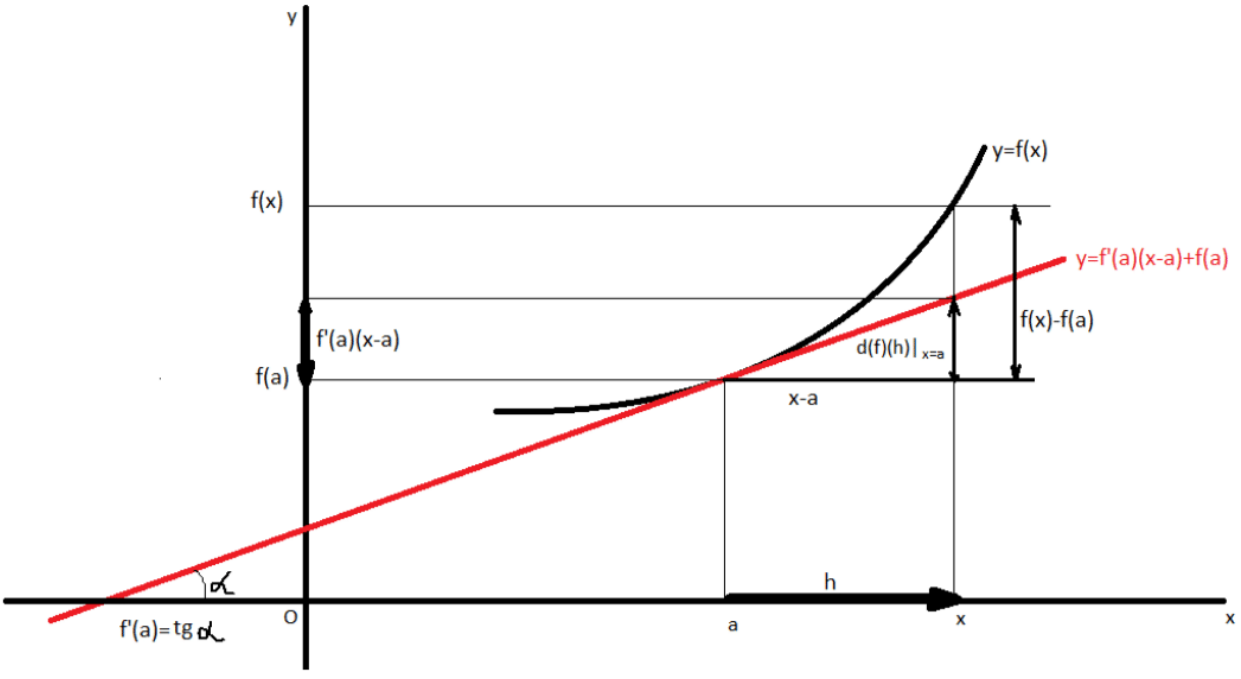
\includegraphics[scale=0.45]{Касательная.png}}
    \caption{Функция "сливается" с касательной.}
    \label{fig:image}
\end{figure} Обратим внимание, что
график функции и касательной неразличимы
в некоторой окрестности.
Приведём несколько примеров на вычисление
производных с помощью определения производной.

\newpage
\begin{problem}
Непрерывность дифференцируемой функции. Определение равномерной сходимости.
\end{problem}

\begin{proposition}
    Пусть функция $f$ дифференцируема
    в точке $a.$ Тогда $f$ непрерывна в точке $a.$
\end{proposition}
\begin{definition}
    Функциональная последовательность
    $\{f_n(x)\}_{n = 1}^\infty$
    \textbf{сходится равномерно} к функции $f(x)$
    на множестве $X$, если
    $$\forall \varepsilon > 0 \ \exists N
        \in \mathbb N: \ \forall n > N \ \forall x \in X
        \ |f_n(x) - f(x)| < \varepsilon.
    $$
    Обозначение: $f_n(x) \underset{X}\rightrightarrows f(x).$
\end{definition}

\newpage
\begin{problem}
Формулировка теоремы о равномерной сходимости последовательности непрерывных
функций. Пример Вейерштрасса непрерывной, но недифференцируемой функции.
\end{problem}
\begin{theorem} (\textbf{Непрерывность предела
        равномерно сходящейся последовательности}).
    Пусть $X$ -- область сходимости
    функциональной последовательности
    $\{f_n\}.$
    Пусть $\forall n \in \N \ f_n(x) \in C(x_0), \ x_0\in X.$
    Пусть $f_n(x) \underset{X}\rightrightarrows f(x).$
    Тогда $f(x) \in C(x_0).$
\end{theorem}
С помощью теоремы о непрерывности предела равномерно
сходящейся последовательности можно построить пример
функции, которая в каждой точке непрерывна,
но ни в одной точке не является дифференцируемой.
Для этого рассмотрим следующую последовательность
функций:
\begin{multline*}
    f_0(x) = \sin x, \ f_1(x) = \sin x + \frac{1}{2} \sin 8x,
    \ f_2(x) = \sin x + \frac{1}{2} \sin 8x +
    \frac{1}{4} \sin 64x, \ ...,\\
    f_n(x) = \sum\limits_{k=0}\limits^{n}\frac{1}{2^k} \sin 8^k x.
\end{multline*}
Покажем, что эта последовательность функций имеет предел
при каждом $x\in\R,$ то есть областью сходимости
является вся вещественная прямая.
Действительно, при фиксированном $x$
$$
    \sum\limits_{k=0}\limits^{n}\left|\frac{1}{2^k}
    \sin 8^k x\right|\leq
    \sum\limits_{k=0}\limits^{n}\frac{1}{2^k}\leq2,
$$
то есть частичные суммы ряда
$\sum\limits_{k=0}\limits^{+\infty}
    \left|\frac{1}{2^k} \sin 8^k x\right|$ ограничены
сверху, что по критерию сходимости для рядов
с положительными коэффициентами означает
сходимость ряда $\sum\limits_{k=0}
    \limits^{+\infty}\left|\frac{1}{2^k} \sin 8^k x\right|,$
то есть ряд $\sum\limits_{k=0}\limits^{+\infty}
    \frac{1}{2^k} \sin 8^k x$ сходится абсолютно, а значит,
и сам этот ряд сходится, то есть по определению
сходится его последовательность частичных сумм
$\{f_n(x)\}_{n=0}^{+\infty}.$
Так как наши рассуждения справедливы для любого
$x\in\R,$ то функция
$$
    w(x) = \sum_{k=0}^\infty \frac{1}{2^k} \sin (8^k x)
$$
определена для любых вещественных чисел.
Кроме того,
$$
    |w(x)-f_n(x)|=\left|\sum\limits_{k=n+1}\limits^{+\infty}
    \frac{1}{2^k} \sin 8^k x\right|\leq
    \sum\limits_{k=n+1}\limits^{+\infty}
    \frac{1}{2^k}=\frac{1}{2^n},
$$
поэтому для каждого $\varepsilon>0$
существует такое $N=[\log_2(1/\varepsilon)],$
что при всех $n>N$ и при всех $x\in\R$
$|w(x)-f_n(x)|<\varepsilon,$ то есть
$f_n(x) \underset{X}\rightrightarrows w(x).$
Все функции $f_n(x)$ непрерывны, так как
представляют собой суммы непрерывных синусов,
поэтому по теореме 1 $w(x)$ непрерывна.

Можно доказать, что при этом функция $w(x)$
ни в одной точке вещественной оси не является
дифференцируемой.

Функция $w(x)=\sum\limits_{n=0}\limits^{\infty}
    2^{-n}\sin(8^nx)$ называется
\textbf{функцией Вейерштрасса.}

\newpage

\begin{problem}
Формулировка правил дифференцирования. Теорема о производной сложной функции.
\end{problem}
\begin{proposition}
    Пусть функции $f$ и $g$ дифференцируемы
    в точке $a.$ Тогда:\\
    1) функция $\alpha f+\beta g$ дифференцируема
    в точке $a$ при любых $\alpha,\;\beta\in \R$
    и $$(\alpha f+\beta g)'(a)=
        \alpha f'(a)+\beta g'(a)$$
    (свойство линейности);\\
    2) $f\cdot g$ дифференцируема в точке $a$
    и $(f\cdot g)'(a)=f'(a)g(a)+f(a)g'(a)$
    (правило Лейбница); \\
    3) если $g\neq0$ в некоторой окрестности
    точки $a,$ то  $\frac{f}{g}$ дифференцируема
    в точке $a$ и $\left(\frac{f}{g}\right)'(a)=
        \frac{f'(a)g(a)-g'(a)f(a)}{g^2(a)}.$
\end{proposition}
\begin{proposition}
    \textbf{(Производная сложной функции).}
    Пусть функция $f$ дифференцируема в точке
    $a,$ а функция $g$ дифференцируема в точке
    $f(a).$ Тогда функция $g\circ f$ дифференцируема
    в точке $a$ и $(g\circ f)'(a)=g'(f(a))\cdot f'(a).$
\end{proposition}

\newpage

\begin{problem}
Инвариантность формы первого дифференциала. Теорема о производной обратной
функции.
\end{problem}
Пусть
$f$ дифференцируема в точке $x$
и $f(x)=y.$ Теорема
о производной сложной функции тогда
в терминах дифференциалов запишется
так (в точке $x$):
$$
    d(g\circ f)(x)=g'(f(x))f'(x)dx=
    g'(f(x))df(x)=g'(y)dy.
$$
Таким образом, вне зависимости от того, является
ли $y$ независимой переменной или функцией,
форма (то есть вид) первого дифференциала
внешне не меняется. Это свойств
дифференциала называется
\textbf{\emph{инвариантностью формы первого
        дифференциала.}}

\begin{proposition}
    \textbf{(Производная обратной функции).}
    Пусть $f$ -- непрерывная и строго монотонная функция,
    отображающая интервал $I$ в интервал $J.$ Пусть также
    $f$ дифференцируема в точке $a\in I$ и $f'(a)\neq0.$
    Тогда обратная функция $f^{-1}$ дифференцируема
    в точке $b=f(a)$ и $(f^{-1})'(b)=\frac{1}{f'(a)}.$
\end{proposition}

\newpage

\begin{problem}
Таблица производных.
\end{problem}
\begin{multline*}
    {\bf 1)} \ C'=0\;\forall C=const; \ {\bf 2)} \ (x^{\alpha})'=
    \alpha x^{\alpha-1}; \ {\bf 3)} \ (e^x)'=e^x; \ {\bf 4)} \ (a^x)'=
    a^x\ln a; \ {\bf 5)} \ (\ln x)'=1/x;\\
    {\bf 6)} \ (\log_a x)'=
    \frac{1}{x\ln a}; \ {\bf 7)} \ (\sin x)'=\cos x; \
    {\bf 8)} \ (\cos x)'=-\sin x; \ {\bf 9)} \ (\tg x)'=
    \frac{1}{\cos^2x}=\tg^2x+1;\\
    {\bf 10)} \ (\ctg x)'=-\frac{1}{\sin^2x}=-\ctg^2x-1; \
    {\bf 11)} \ (\arcsin x)'=\frac{1}{\sqrt{1-x^2}}; \
    {\bf 12)} \ (\arccos x)'=-\frac{1}{\sqrt{1-x^2}};\\
    {\bf 13)} \ (\arctg x)'=\frac{1}{1+x^2}; \
    {\bf 14)} \ (\arcctg x)'=-\frac{1}{1+x^2}; \
    {\bf 15)} \ (\sh x)'=\ch x; \
    {\bf 16)} \ (\ch x)'=\sh x.
\end{multline*}

\newpage

\begin{problem}
Определения локальных минимума и максимума и локального экстремума. Теорема
Ферма.
\end{problem}
\begin{definition}
    Пусть $\delta>0, U_\delta(a)$ - $\delta$-окрестность точки а Если функция $f$ определена на множестве $E$, точка $a \in E$ и при всех $x \in U_\delta(a) \cap E$, выполнено неравенство $f(x) \geq f(a)$, то а называется точкой локального максимума. Если при тех же $x \in U_\delta(a) \cap E f(x) \leq f(a)$, то $f$ называется точкой локального минимума. Если неравенство строгое, то а называется точкой строгого локального максимума или строгого локального минимума соответственно. Точки максимума и минимума называются точками локального экстремума (если неравенства нестрогие), и точками строгого локального экстремума, если неравенства строгие.
\end{definition}

\begin{theorem}
    (Теорема Ферма). Пусть функиия $f$ определена на интервале $(a, b)$, дифференцируема в точке $c \in(a, b)$ и имеет в точке с локальный экстремум. Тогда $f^{\prime}(c)=0$.
\end{theorem}


\newpage

\begin{problem}
Теорема Ролля. Теорема Лагранжа. Геометрические смыслы этих теорем.
\end{problem}
\begin{theorem}
    (Теорема Ролля), Пусть:\\
    1) Функция $f$ определена и непрерывна на отрезке $[a, b]$.\\
    2) Функция $f$ дифференцируема па иттервале $(a, b)$.
    3) $f(a)=f(b)$.

    Тогда существует такая точка $c \in(a, b)$, что $f^{\prime}(c)=0$.
\end{theorem}

\begin{theorem}
    (Теорема Лагранжа). Пусть:\\
    1) Функция $f$ определена и непрерывна на отрезке $[a, b]$.\\
    2) Функция $f$ дифференцируема па интервале $(a, b)$.

    Тогда существует такая точка $c \in(a, b)$, что $f(b)-f(a)=f^{\prime}(c)(b-a)$.
\end{theorem}

\newpage

\begin{problem}
Два следствия теоремы Лагранжа. Теорема Коши.\end{problem}
\begin{proposition}
    (1-е следствие) Пусть функция $f$ определена и дифференцируема на интервале $(a, b)$ и $f^{\prime}(x)=0 \forall x \in(a, b)$. Тогда функция $f$ постоянна на $(a, b)$.
\end{proposition}

\begin{proposition}
    (2-е следствие) Пусть функция $f$ определена и дифференцируема на интервале $(a, b)$.
    1) Функция $f$ не убывает на этом интервале тогда и только тогда, когда
    $$
        f^{\prime}(x) \geq 0 \forall x \in(a, b) \text {. }
    $$
    2) Функция $f$ не возрастает на этом интервале тогда и только тогда, когда
    $$
        f^{\prime}(x) \leq 0 \forall x \in(a, b) .
    $$
\end{proposition}

\begin{theorem}
    (Теорема Коии). Пусть функции $f$ и $g$ :
    1) определены и непрерывны на отрезке $[a, b]$;
    2) дифферениируемы на интервале $(a, b)$;
    3) $g^{\prime}(x) \neq 0 \forall x \in(a, b)$.

    Тогда существует точка такая точка $c \in(a, b)$, что $\frac{f(b)-f(a)}{g(b)-g(a)}=\frac{f^{\prime}(c)}{g^{\prime}(c)}$.
\end{theorem}
